\subsection{SOlUCIÓN 5}

\subsubsection{Actividad 1 lab 5}
%*********************
\begin{frame}{}

\pgfdeclareimage[width=\paperwidth,height=\paperheight]{bg}{imagenes/fondo_seccion}
\setbeamertemplate{background}{\pgfuseimage{bg}}

\definecolor{greenU}{RGB}{212,202,72}
\setbeamercolor{block body}{fg=Black,bg=greenU}
\begin{block}{}
	\centering
	\vspace{1mm}
	\large{\textit{solucion lab 5 actividad 1}}
	\vspace{1mm}
\end{block}
\end{frame}


\begin{frame}{Solución de la actividad "Modificación del parámetro alpha en un filtro de coseno realzado"}
\begin{figure}
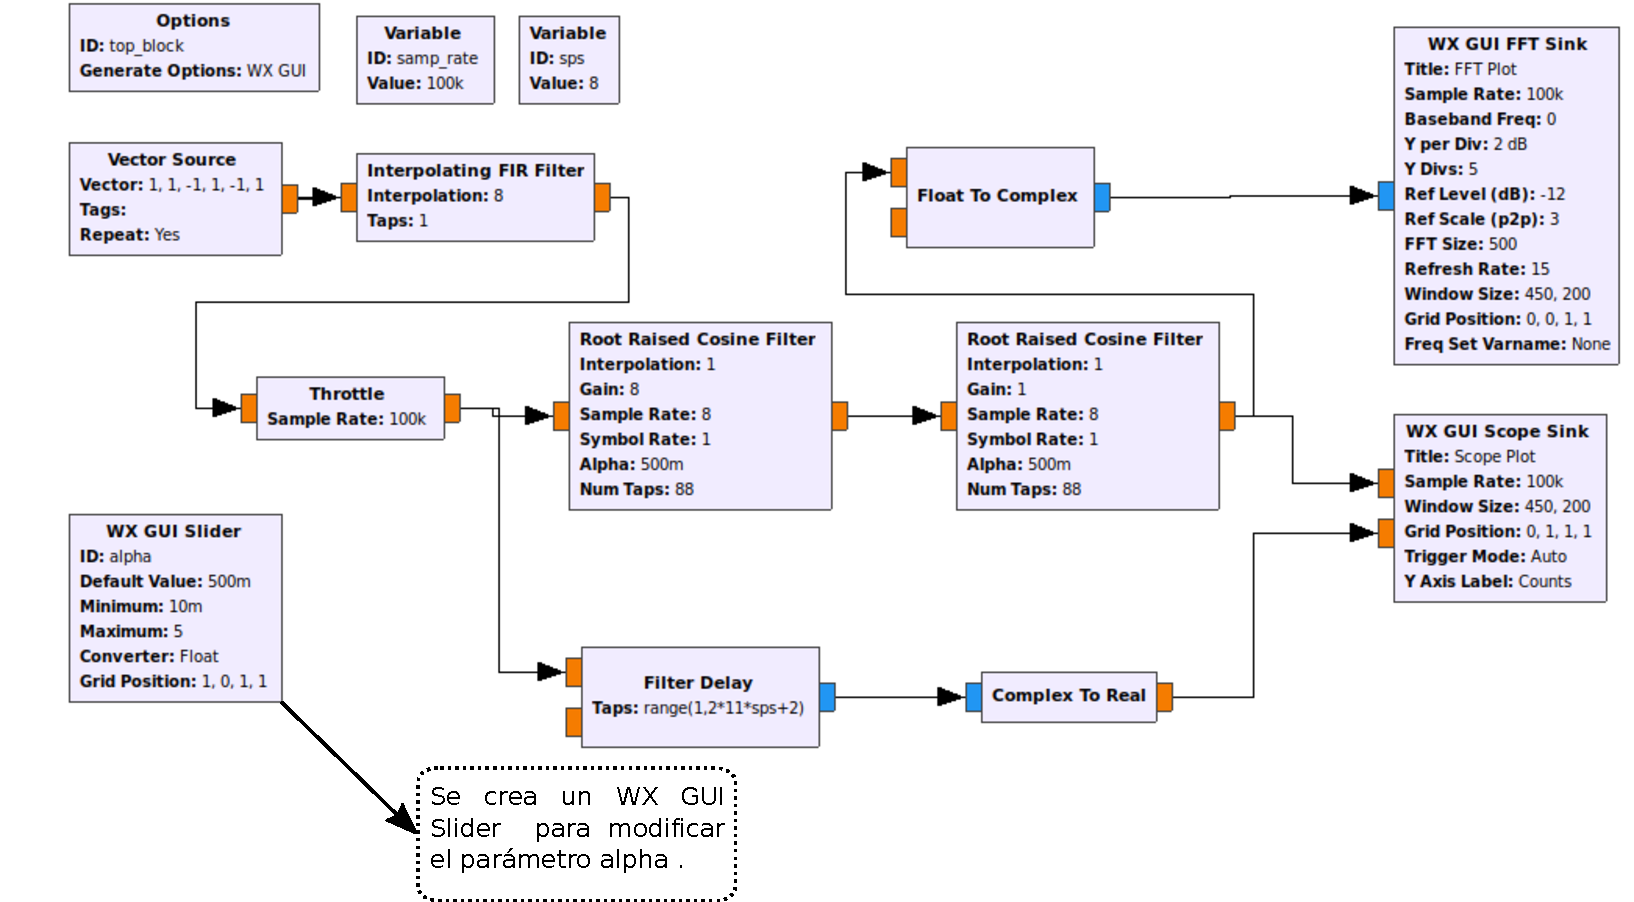
\includegraphics[width=.9\textwidth]{soluciones/actividad-5-1/pdf/lab5_7.pdf}
\end{figure}
\end{frame}
%-------------------------------------------------------------------------------    
\begin{frame}{Solución de la actividad "Modificación del parámetro alpha en un filtro de coseno realzado"}
$$\alpha=0.5$$
\begin{figure}
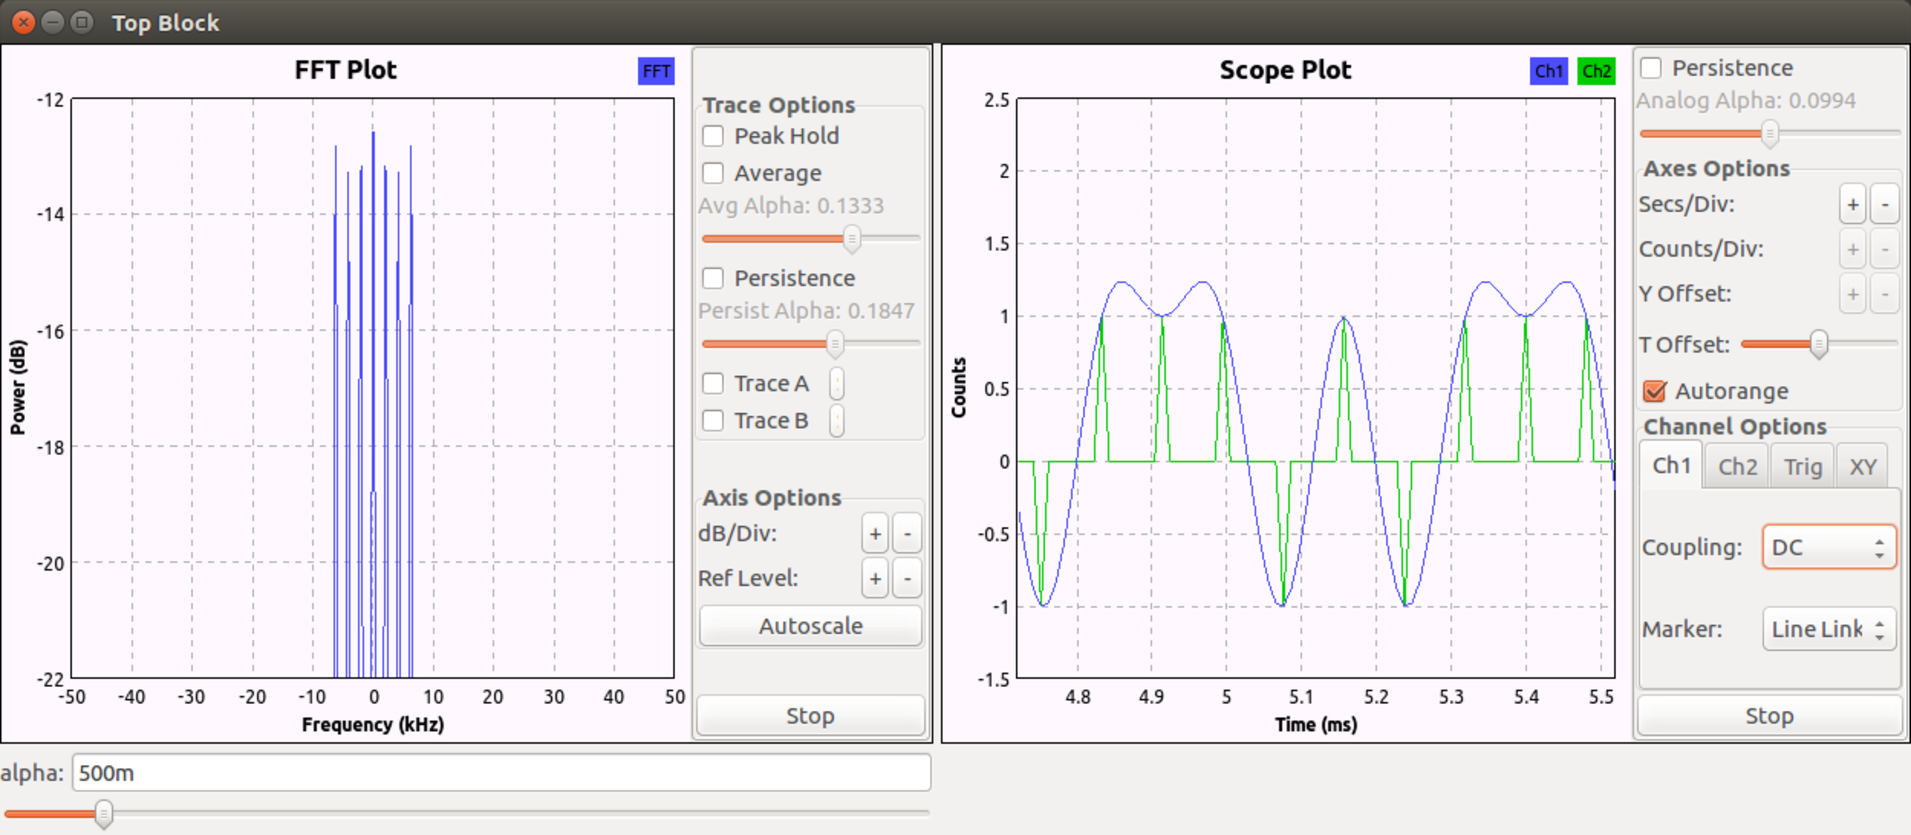
\includegraphics[width=1.05\textwidth]{soluciones/actividad-5-1/pdf/lab5_8.pdf}
\end{figure}
\end{frame}
%--------------------------------------------------------------------------
\begin{frame}{Solución de la actividad "Modificación del parámetro alpha en un filtro de coseno realzado"}
$$\alpha=1.35$$
\begin{figure}
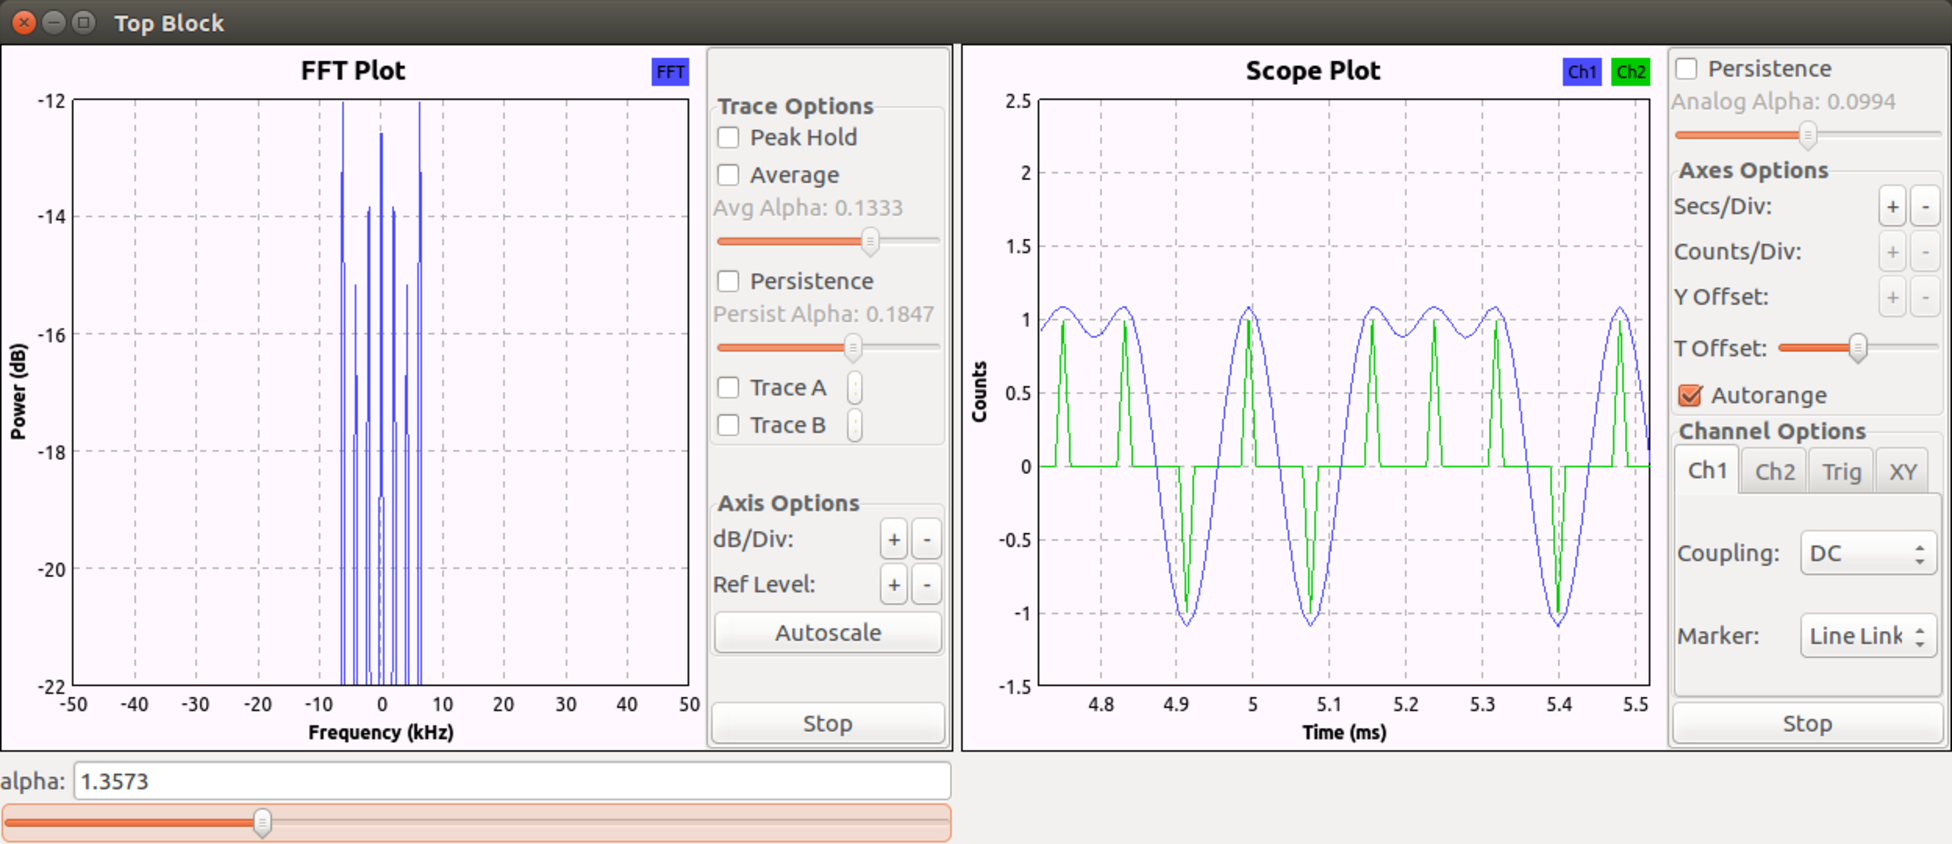
\includegraphics[width=1.05\textwidth]{soluciones/actividad-5-1/pdf/lab5_9.pdf}
\end{figure}
\end{frame}
%----------------------------------------------------------------------------
\begin{frame}{Solución de la actividad "Modificación del parámetro alpha en un filtro de coseno realzado"}
$$\alpha=3.25$$
\begin{figure}
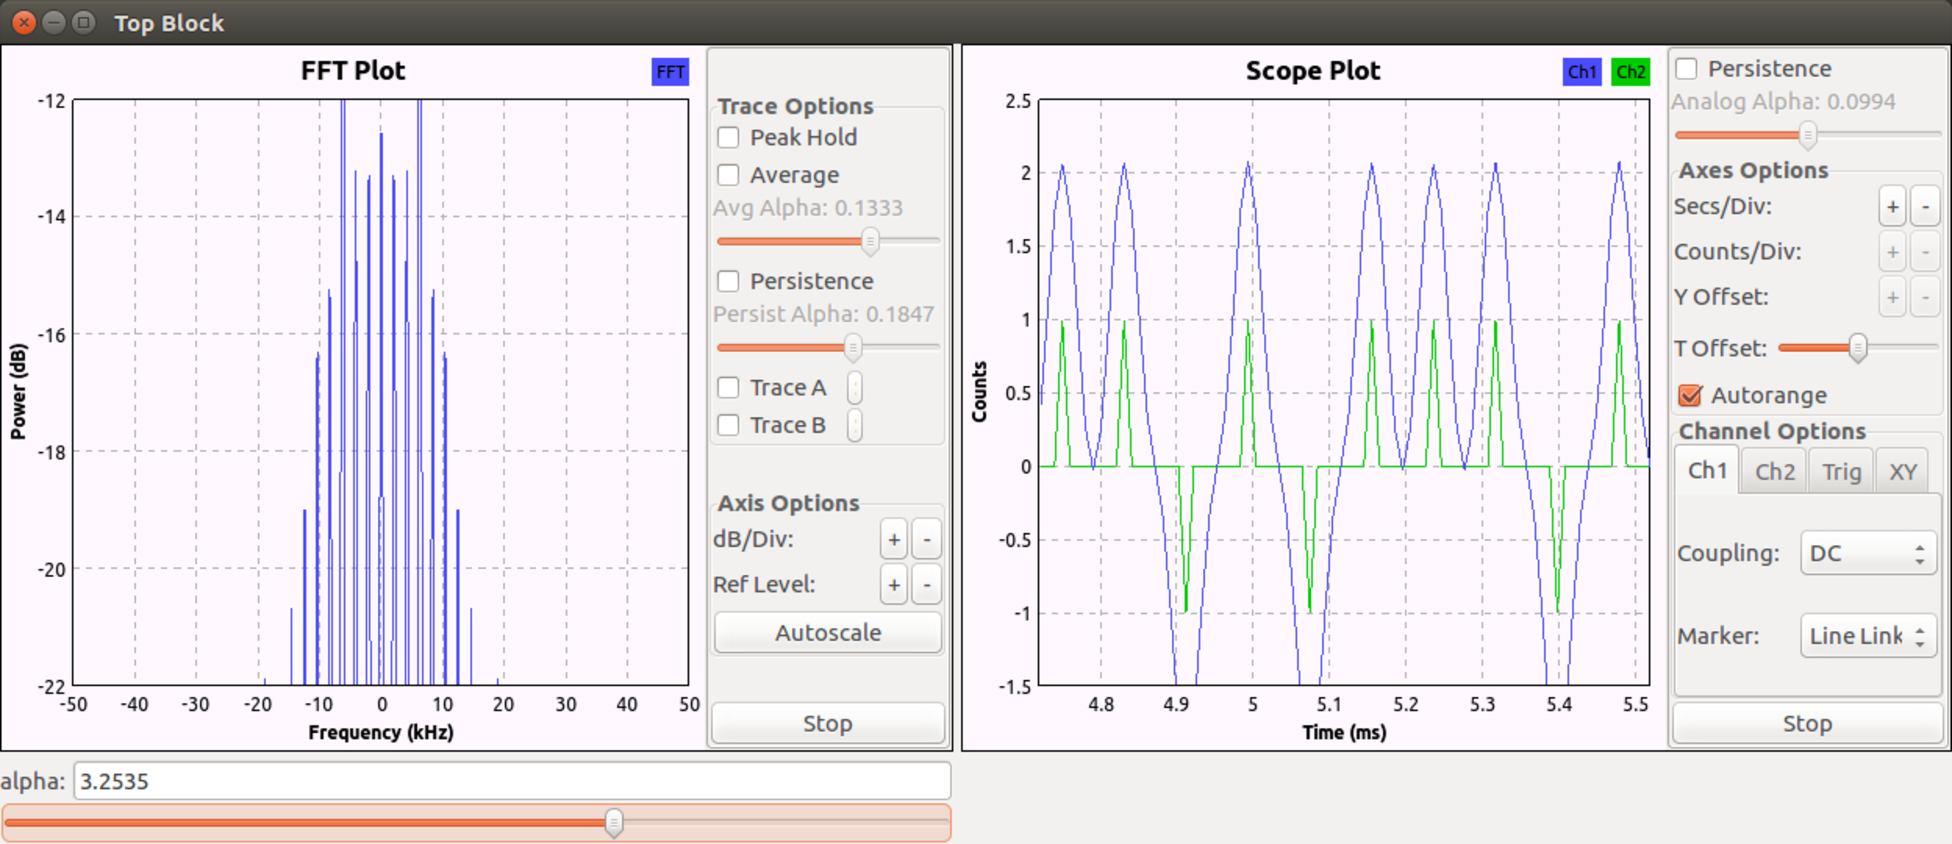
\includegraphics[width=1.05\textwidth]{soluciones/actividad-5-1/pdf/lab5_10.pdf}
\end{figure}
\end{frame}
%-----------------------------------------------------------------------------
\begin{frame}{Solución de la ctividad "Modificación del parámetro alpha en un filtro de coseno realzado"}
\justifying
Como se puede observar , cuando el valor de $\alpha$ sobrepasa 1, la potencia de las bandas laterales supera la de la portadora , causando que la señal aumente la amplitud y la forma de esta se parezca cada vez mas al tren de pulsos representado por el canal 2. Así mismo si se aumenta mucho el parámetro $\alpha$ se ve afectado el ancho de banda puesto que este aumenta.
\end{frame}